\documentclass[10pt, a5paper]{article}

%-----------------------------------------------------------------
%       DO NOT EDIT THIS DOCUMENT WITHOUT PERMISSION
%-----------------------------------------------------------------

\usepackage[utf8]{inputenc}
\usepackage{amsmath}
\usepackage{amssymb}
\usepackage{amsthm}
\usepackage{algorithm}
\usepackage{algpseudocode}
\usepackage{array}
\usepackage{booktabs}
\usepackage{bchart}
\usepackage{csquotes}
\usepackage{caption}
\usepackage{color}
\usepackage{comment}
\usepackage{csvsimple}
\usepackage{enumitem}
\usepackage{eurosym}
\usepackage{fancyref}
\usepackage[bottom]{footmisc}
\usepackage{fancyhdr}
\usepackage{float}
\usepackage{hyperref}
\usepackage{listings}
\usepackage{longtable}
\usepackage{mathtools}
\usepackage{makecell}
\usepackage{multirow}
\usepackage{multicol}
\usepackage{pdfpages}
\usepackage{ragged2e}
\usepackage[figuresright]{rotating}
\usepackage{sidecap}
\usepackage{svg}
\usepackage{tabularx}
\usepackage{times}
\usepackage[colorinlistoftodos]{todonotes}
\usepackage{textcomp}
\usepackage{silence}
\usepackage{lipsum}
\usepackage[lmargin=1.5cm, rmargin=1.5cm, tmargin=2cm, bmargin=2cm]{geometry}
\usepackage{parskip}

\definecolor{codegreen}{HTML}{116611}
\definecolor{codegray}{HTML}{666666}
\definecolor{codeblue}{HTML}{0066CC}
\definecolor{backcolour}{HTML}{f6f6f6}
\lstdefinestyle{shiftstyle}{
  backgroundcolor=\color{backcolour},
  commentstyle=\color{codegray},
  keywordstyle=\color{codeblue},
  numberstyle=\tiny\color{codegray},
  stringstyle=\color{codegreen},
  basicstyle=\ttfamily\footnotesize,
  breakatwhitespace=false,         
  breaklines=true,                 
  captionpos=b,                    
  keepspaces=true,                 
  numbers=left,                    
  numbersep=5pt,                  
  showspaces=false,                
  showstringspaces=false,
  showtabs=false,                  
  tabsize=2
}
\lstset{style=shiftstyle}

\pagestyle{fancy}
\fancyhf{}
\lhead{
\includegraphics[height=0.6cm]{images/logo_header.png}}
\rfoot{\thepage}
\lfoot{Study Tour Shift 2018 -- University of Twente}
\setlength{\headheight}{21pt}
\renewcommand{\footrulewidth}{0.4pt}
\setcounter{secnumdepth}{3}
\setcounter{tocdepth}{3}


\usepackage{pgfplots, pgfplotstable}
\usepackage{filecontents}
\usepackage{subcaption}



\pgfplotsset{compat=1.7}

%% Code chunk for statistics starts here...
\newcommand{\calcrowmean}{
    \def\rowmean{0}
    \pgfmathparse{\pgfkeysvalueof{/pgfplots/table/summary statistics/end index}-\pgfkeysvalueof{/pgfplots/table/summary statistics/start index}+1}
    \edef\numberofcols{\pgfmathresult}
            % ... loop over all columns, summing up the elements
    \pgfplotsforeachungrouped \col in {\pgfkeysvalueof{/pgfplots/table/summary statistics/start index},...,\pgfkeysvalueof{/pgfplots/table/summary statistics/end index}}{
        \pgfmathparse{\rowmean+\thisrowno{\col}/\numberofcols}
        \edef\rowmean{\pgfmathresult}
    }
}
\newcommand{\calcstddev}{
    \def\rowstddev{0}
    \calcrowmean
    \pgfplotsforeachungrouped \col in {\pgfkeysvalueof{/pgfplots/table/summary statistics/start index},...,\pgfkeysvalueof{/pgfplots/table/summary statistics/end index}}{
        \pgfmathparse{\rowstddev+(\thisrowno{\col}-\rowmean)^2/(\numberofcols-1)}
        \edef\rowstddev{\pgfmathresult}
    }
    \pgfmathparse{sqrt(\rowstddev)}
}
\newcommand{\calcstderror}{
    \calcrowmean
    \calcstddev
    \pgfmathparse{sqrt(\rowstddev)/sqrt(\numberofcols)}
}

\pgfplotstableset{
    summary statistics/start index/.initial=1,
    summary statistics/end index/.initial=10,
    create col/mean/.style={
        /pgfplots/table/create col/assign/.code={% In each row ... 
            \calcrowmean
            \pgfkeyslet{/pgfplots/table/create col/next content}\rowmean
        }
    },
    create col/standard deviation/.style={
        /pgfplots/table/create col/assign/.code={% In each row ... 
            \calcstddev
            \pgfkeyslet{/pgfplots/table/create col/next content}\pgfmathresult
        }
    },
    create col/standard error/.style={
        create col/assign/.code={% In each row ... 
            \calcstderror
            \pgfkeyslet{/pgfplots/table/create col/next content}\pgfmathresult
        }
    }
}
%%...code chunk for statistics ends here






\begin{document} 

\title{Automatic DDoS Attack Rule Generation for SIDS applied to BRO}
\author{René Boschma\\University of Twente\\r.boschma@student.utwente.nl}
\date{}
\maketitle

% You should not remove or rename these sections
% You should not remove this section
\section*{Abstract}
\label{section:abstract}
A Distributed Denial of Service (DDoS) attack aims to disable services of a target system using multiple machines. As the number of attacks increase and downtime costs are exceeding on
average \$300K per hour [1] a need for an efficient and effective mitigation method has become crucial. Our hypothesis is that Signature-based Intrusion Detection system is a suitable system that can detect DDoS attacks when their downside of keeping an up-to-date signature list is tackled. In this paper, we will implement automatic signature generation for Bro. We will test these signatures by replaying various DDoS attack vectors retrieved from DDoSDB against a common network architecture.  

In this paper, we show that it is possible for the selected attack vectors to automatically generate Bro signature within 4.2 milliseconds. Also that Bro is capable of detecting and responding to all attacks within 0.31 milliseconds when only one signature is active and within 0.7 milliseconds with all our generated signatures.
\newpage
% You should not remove this section
\section{Introduction}
\label{section:introduction}
A Denial of Service (DoS) attack is an attack that aims to disable services of a target system. There are two main types of DoS attacks: \textit{vulnerability DoS} and \textit{flood DoS} \cite{Lin2013}. In one hand, a vulnerability DoS aims to exploit a vulnerability of a target system to reduce its performance or render it useless. An example of such an attack is to send a malformed message to the target machine which can not deal with this message and as a result stops working. On the other hand, a flood DoS attack tries to exhaust the resources of the target. An example of such an attack is to fill the entire bandwidth of the target with messages of the attacker. The attacker can accomplish such bandwidth flood by using multiple machines to produce traffic. When multiple machines are used in the attack, it is called a Distributed Denial of Service (DDoS) attack.  



%An explanation for this increase in frequency could be the rise of \textit{booters} \cite{Santana2017}. A booter, also called stressers, are websites that offer DoS attacks via a website. Booters eliminate the need for any technical knowledge to launch an attack. Clients of booters only need to pay a couple of dollars to launch an attack.

DDoS attacks have increased in power and frequency. In 2011, the peak attack was measured at 60 Gb/s \cite{Arbor2014}, in 2015, 500 Gb/s and in 2016 1.1 Tb/s \cite{Akamai2017}. In the third quartile of 2016 more than 5000 attacks where observed, whereas 200 in the entire 2012 \cite{Akamai2016}. As the number of attacks increase and downtime costs are exceeding on average \$300K per hour \cite{ITIC2016} a need for an efficient and effective mitigation method has become crucial. The first task before the mitigation is the detection of an attack. Intrusion Detection Systems (IDSs) are such systems that can fulfill this task. An IDS is a system that monitors a system or network for malicious and/or suspicious activities. 
%Two main categories of IDSs are present: \textit{host-based} and \textit{network-based} \cite{Fallahi2016}. A Host-based IDS (HIDS) is only for a single machine. A Network-based IDS (NIDS) is for an entire network. A NIDS usually scans the incoming and outgoing traffic of a network endpoint. 
Based on the detection methods of IDSs, two categories can be identified: \textit{Anomaly-based} and \textit{Signature-based} \cite{fragkiadakis2015anomaly}. An Anomaly-based IDS (AIDS) bases its detection on a constructed baseline and detects deviations from this baseline. A Signature-based IDS (SIDS) bases its detection on key characteristic of an attack for which predefined signatures are known. An AIDS has as benefit that it can detect unknown attacks but with the weaknesses that it has a low accuracy, needs time to learn a baseline of a system and has difficulties to trigger alerts before an attack scales up. A SIDS has as benefit that it has a high accuracy but with the weaknesses that it is ineffective in detecting unknown attacks and it is hard to maintain an up to date signature list \cite{Liao2013}. 

Our hypothesis is that due to the high accuracy a SIDS is a suitable system that can fulfill the requirement of successfully and efficiently detecting DDoS attacks when the major downside of keeping an up to date signature list is tackled. The solution for this problem is to generate signatures for new attacks. This can be done either manually or automatically. As a manual approach requires significant amount of manual effort \cite{Lin2013}, we propose an automatic method. For this research we generate rules from extracted features of DDoS attacks for the Bro SIDS\footnote{\url{https://www.bro.org/}}. Bro is an open source network security monitor that offers the functionality of a SIDS. The features of DDoS attacks are extracted by a different research of DDoSDB\footnote{\url{http://ddosdb.org/}}.

%We apply the to generate signatures and apply this to specific SIDS. We have chosen Bro\footnote{\url{https://www.bro.org/}} as SIDS. Bro is an open source network security monitor that offers the functionality of a SIDS. 



To pursue our goal we have defined the following research questions (RQ) as the basis of the proposed research:

%Intrusion Detection Systems (IDS) is a system that monitors a network or system for malicious and/or suspicious activities within a network or system. Two main cattogories of IDSs are present: \textit{host-based} and \textit{network-based} \cite{Fallahi2016}. A Host-based IDS (HIDS) is only for a single machine. A Network-based IDS (NIDS) is for an entire network. A NIDS usually scans the incoming and outgoing traffic of a network endpoint. Based on the detection methods of IDSs, again two categories can be identified: \textit{Anomaly-based} and \textit{Signature-based} \cite{fragkiadakis2015anomaly}. An Anomaly-based IDS (AIDS) bases its detection on a constructed baseline and detects deviations from this baseline. A Signature-based IDS (SIDS) bases its detection on signatures. An AIDS has as benefit that it can detect unknown attacks but with the weakness that it has a low accuracy and difficulty to trigger alerts in the right time. A SIDS has as benefit that it has a high accuracy but with the weakness that it is ineffective in detecting unknown attacks and it is hard to maintain an up to date signature list \cite{Liao2013}. 



%As the number of attacks are increasing and downtime costs are exceeding on average \$300K per hour \cite{ITIC2016} a need for an efficient and effective mitigation method becomes bigger. We believe that SIDSs are promising systems that can fulfil these requirements when the major downside of keeping and up to date signature list is tackled. That is why we propose an automatic method to generate signatures for the SIDS Bro\footnote{\url{https://www.bro.org/}}. To accomplish this goal we have defined the following research questions (RQ):

\begin{itemize}	
	\item \textbf{RQ1:} What are the DDoS characteristics that could be used for generating BRO detection/mitigation rule?
	\item \textbf{RQ2:} What is the performance of automatic rule generation against a DDoS attack for the Bro SIDS?
	 \item \textbf{RQ3:} What is the efficiency for Bro automatic generated rules when applied on an ongoing DDoS attack?
\end{itemize}

The first RQ will be answered by analyzing the most common DDoS attack vectors described by Akami \cite{Akamai2017-4}. The second RQ will be answered by building a proof of concept that generates signatures based on a given stream of features of DDoS attacks. The third and last RQ will be answered by replaying an attack for which a signature was generated and analyze what the performance of Bro is with these signatures implemented. 





%\comment{The Introduction section has more or less the same structure as your abstract. The difference is that in the abstract each part is one statement/phrase, while in the introduction each part is a paragraph. So, (i) context, (ii) problem, (iii) proposal, and your most astonishing (iv) finding. Of course in the Introduction section you can give far more details than in the abstract. Avoid to copy and paste statements, re-write with different words.}

%\comment{In addition to the structure that you already know you should include your \textit{research questions} between the ``proposal'' paragraph and the ``findings''. The statement that precede the RQ is something like the following: }

%``To pursue our goal, we have defined the following research questions (RQ) as the basis of our research: 


%\comment{Please, avoid "yes or no" questions. Make questions that your reader are not able to answer immediately. Usually the questions depend on each other, it means that to answer one question you must answer the one before.}

%\comment{Before a little bit of your most astonishing findings you must to introduce the structure of your paper/proposal. Usually the text looks like the following.}
 


% Your sections should be here, you are free to change, add and remove any section here that you see fit.
\section{Content}
\label{section:content}

\subsection{DDoS Attacks and BRO}\label{subsec:ddos-and-bro}
In this section we will first define the notion of a DDoS attack by explaining how the infrastructure looks like. Then we will elaborate on various DDoS attacks used nowadays and discuss their main characteristics. After this we will discuss the syntax of the detection rules of the BRO SIDS.

\subsubsection{The DDoS Attack}
Figure \ref{fig:ddos-overview} shows the infrastructure of a DDoS attack. Actors involved in a DDoS attack are denoted by a letter (A-D) whereas data streams are denoted by numbers (1-5). 

A DDoS attack starts with an attacker (A). The attacker sends data needed to start the attack (1) to the Command and Control (C\&C) servers (B). The C\&C servers control the infected machines (C). The infected machines are also known under the name of bots. The C\&C servers plus the infected machines are more commonly named as a botnet. The C\&C servers send a message (2) to the infected machines. In case of the Ramnit botnet, only the infected machines counted 3.2 million machines \cite{europol2015}. At this point two paths are used to get to the target machine (E). The first path possible is aiming the infected machines directly to the target (4). The second path possible is using public services (D) like a DNS to reach the target (5). 

In the next subsection we will describe various types of DDoS attacks. 

\begin{figure}[H]
\centering
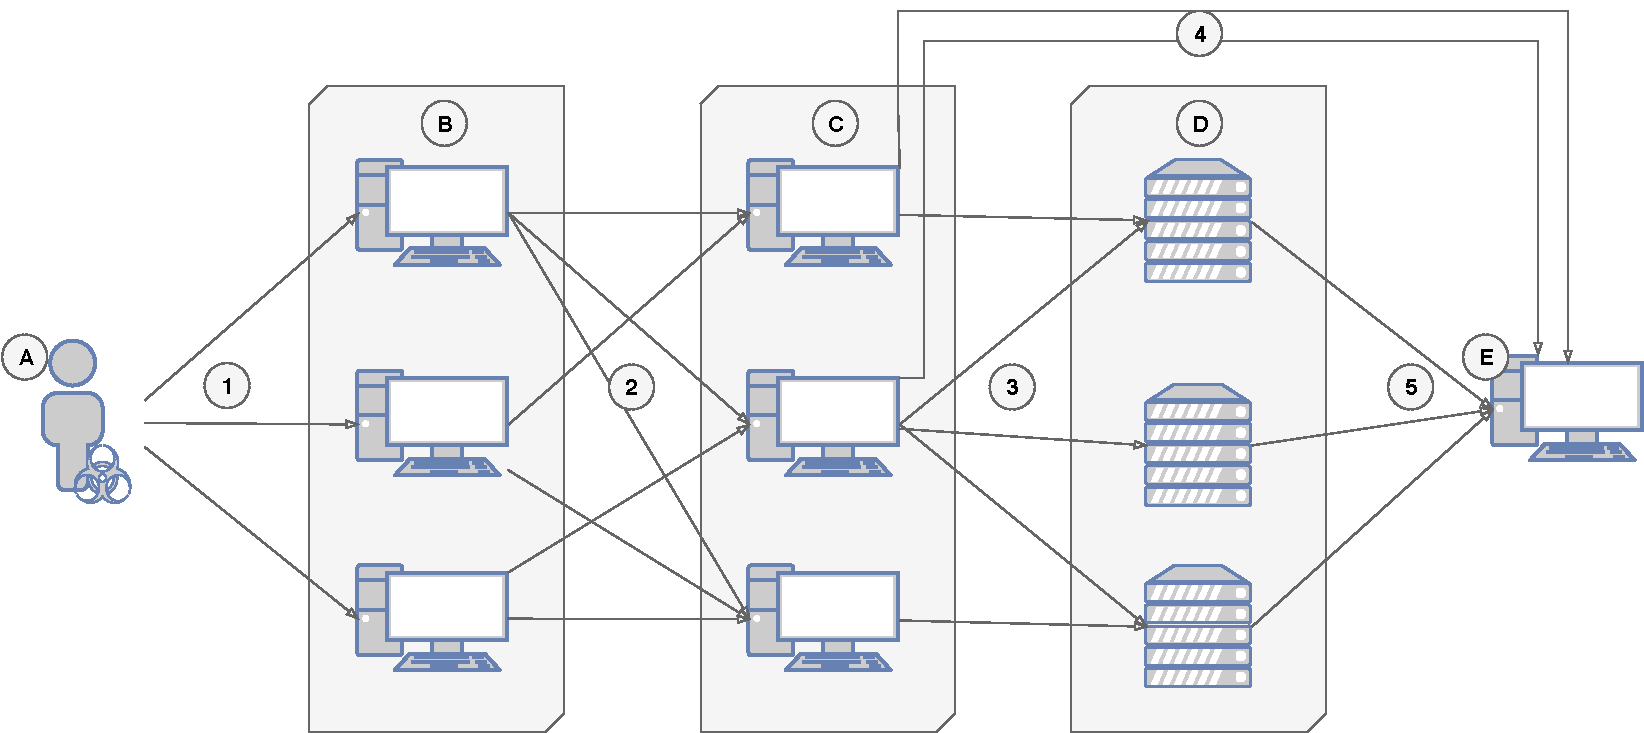
\includegraphics[width=\textwidth]{./images/ddos-overview.pdf}
\caption{Overview of DDoS attack infrastructure}
\end{figure}\label{fig:ddos-overview}

\subsubsection{Types of Attacks}
In this section we will briefly elaborate on various types of attack. The main characteristics can be found in Table $\dots$.

\paragraph{UDP Fragment}



\subsubsection{BRO Rule Syntax} 


\subsection{Methodology}\label{subsec:methodology}

\subsection{Evaluation and Discussion}\label{subsec:evaluation-discussion}
\subsubsection{Evaluation}\label{subsubsec:evalutation}
\subsubsection{Discussion}\label{subsubsec:discussion}


% You should not remove or rename this section
% You should not remove this section
\section{Conclusion}
\label{section:conclusion}
In this paper we try to show whether Bro is a suitable IDS which is capable of detecting attacks with automated generated rules based on the signatures retrieved from DDoSDB. We tried to show this by building a test setup that resembles a common internet setup. In this setup we replayed various attack vectors to a target machine which port was mirrored to a machine running the Bro IDS. 

From this we can conclude that (1) it is possible to automatically generate Bro signature rules based on signatures received from DDoSDB, (2) generation time of the signature rules is based on the number of fields the signature has and (3) Bro's response time does not increase dramatically when more signatures are added. 

For future work one could look at the Bro scripting language. The Bro scripting language allows for more detailed analisys of packets. Also one could increase the number of signatures to discover the limit of signatures the Bro IDS can handle. Furthermore, it would also be nice to see how the generated rules behave in terms of accuracy (false positives and false negatives). 

\section{Acknowledgements}
We would like to thank Jair Santanna for his valuable feedback, supplying the tools needed for the test setup and enabling us to gain access to the data stored in DDoSDB. Furthermore, We would like to thank Vincent Dunning for aiding in the process of creating the test setup and carrying out the experiments.  

\newpage
\bibliographystyle{plain}
\bibliography{./references}

\end{document}